\documentclass[11pt]{article}
\usepackage[margin=1in]{geometry}
\usepackage{amsmath, amssymb, amsthm}
\usepackage{bm}
\usepackage{graphicx}
\usepackage{booktabs}
\usepackage{microtype}
\usepackage{xcolor}
\usepackage{url}
\usepackage[hidelinks]{hyperref}

\newtheorem{proposition}{Proposition}
\newtheorem{lemma}{Lemma}
\newtheorem{corollary}{Corollary}
\theoremstyle{definition}
\newtheorem{definition}{Definition}
\theoremstyle{remark}
\newtheorem{remark}{Remark}

\newcommand{\DAVIS}{\textsc{Davis}}
\newcommand{\GIGI}{\textsc{GIGI}}
\newcommand{\BW}{\textsc{BW05}}
\newcommand{\RR}{\mathbb{R}}
\newcommand{\Hb}{\mathbb{H}}
\newcommand{\T}{\mathcal{T}}
\newcommand{\cR}{\mathcal{R}}
\newcommand{\ip}[2]{\langle #1,\,#2\rangle}
\newcommand{\norm}[1]{\lVert #1\rVert}
\newcommand{\Pone}{\mathcal{P}_1^{\mathrm{cl}}}

\title{Redundancy as Stabilizer:\\[2pt]
\large A Consistent, Coercive Petrov--Galerkin Curvature Force\\ for Discrete Yang--Mills Dynamics on the Poincar\'e Homology Sphere}
\author{Bee Rosa Davis\\ \small Davis Geometric}
\date{November 2026}

\begin{document}
\maketitle

\begin{abstract}
The \DAVIS{}--Wilson programme asks whether lattice gauge dynamics computed from coarse
edge data reproduce the continuum geometric flow they discretize. In the exact
instantaneous form that matters for the programme, the discrete force evaluated on the
exact edge integrals of a smooth connection, tested against \emph{every} discrete
variation, must converge to the continuum force. For the lowest-order Whitney
discretization this fails: on a sequence of shape-regular meshes of the Poincar\'e
homology sphere $S^3/2I$, the relative force error of an Abelian control stalls at
$26\%$ under refinement.

We show that this floor is a property of how curvature is \emph{represented}, not of the
data, and that it can be removed without sacrificing stability. A closed linear
curvature recovered on each cell's face-star, tested against the original Whitney
variations, gives a Petrov--Galerkin force that is consistent. In its minimal
(one-ring) form, however, the recovery is exactly determined. It interpolates rough data
as large linear fields, with a per-cell amplification of $125$--$254$, and the resulting
operator has thousands of eigenvalues with negative real part.

Recovering on a \emph{two-ring} neighbourhood by equality-constrained least squares keeps
the recovery exact on closed linear curvature, cuts the amplification to a mesh-uniform
$31$--$47$, and changes the operator's character completely. The relative force error
falls to $6.22\%$, $3.83\%$, $2.79\%$ and $1.45\%$ at $n=1,2,3,5$, with observed orders
$0.73$, $0.80$ and $1.29$. Every physical eigenvalue has positive real part, with the
smallest at the control's true value of $4$. The symmetric part of the operator is
positive definite on the physical space, so the semi-discrete flow is dissipative in the
native mass norm.

No parameter is fitted or tuned. Redundancy in the recovery, not added resolution or
damping, is what stabilizes it. The force is not the gradient of an energy; we
document, quantitatively, why every symmetrized variant we tested fails, and state
precisely what remains open.
\end{abstract}

\section{Introduction}

Lattice gauge theory and geometric flows meet in a single question. Given a smooth
connection $A$ on a closed Riemannian $3$-manifold, and only its integrals along the edges
of a mesh, can a discrete force be computed from that data alone so that it converges to
the continuum Yang--Mills force $-\delta F_A$, uniformly over all discrete variations?
For the homogeneous $SU(2)$ backgrounds of the \DAVIS{}--Wilson programme, a continuum
statement is in hand for a specific class: for positive diagonal left-invariant metrics,
the Ricci velocity mapped through the Levi-Civita connection equals the negative
Yang--Mills gradient exactly, with the clock fixed to one rather than fitted. That
statement is instantaneous and homogeneous. It is not a general Ricci-flow result, and
fixed-background trajectory equivalence fails in the tested non-round cases. Any lattice
realisation of the programme also needs something more basic: a discrete Yang--Mills
force that converges to its continuum counterpart. That prerequisite, for an Abelian
control, is the subject of this paper.

The difficulty is not approximation in the usual sense. The lowest-order Whitney
discretization~\cite{whitney1957,bossavit1988} is a perfectly good finite element method:
its Galerkin solutions converge~\cite{afw2006,afw2010,hiptmair2002}. But the
\emph{instantaneous} question is different. The force is evaluated on the exact edge data
$I_hA$ and tested against every Whitney variation. Here a curvature error of order $h$
meets a test field whose curl is of order $h^{-1}$, and the product is of order one. The
inconsistency of the combinatorial codifferential on unstructured meshes is
known~\cite{afgt2014}; on our meshes it appears as a relative error of $25.9\%$ to
$26.1\%$ that does not decrease under refinement (Table~\ref{tab:force}).

Prior attempts, recorded in the accompanying engineering reports, took two routes, and
each failed one of two requirements:
\begin{itemize}
  \item \emph{Variational} recoveries reconstruct a better curvature and differentiate
    its energy. The energy becomes accurate (density $1.987$ towards $2$), but the
    gradient is wrong by hundreds of percent, because differentiating the reconstruction
    replaces the test variations.
  \item A \emph{Petrov--Galerkin} recovery keeps the original Whitney test variations and
    replaces only the trial curvature. It is consistent, at $1.17\%$ for $n=5$, but its
    operator has eigenvalues with real part as negative as $-2.4\times 10^{4}$.
\end{itemize}

\paragraph{Contributions.}
\begin{enumerate}
  \item An exact decomposition of the instantaneous force error into a
    \emph{reconstruction} term and a \emph{test-variation} term
    (Proposition~\ref{prop:decomp}). It explains, in one identity, the Whitney floor, the
    variational divergence, and the Petrov--Galerkin consistency.
  \item A diagnosis of the Petrov--Galerkin instability as a \emph{conditioning} defect:
    the one-ring recovery is exactly determined, so its amplification of rough data is
    the reciprocal of a small singular value (Section~\ref{sec:conditioning}).
  \item A two-ring, equality-constrained least-squares recovery. It is exact on closed
    linear curvature, has mesh-uniform amplification, and gives a force that passes the
    unchanged \BW{} convergence gate and the stability test. Its symmetric part is
    positive definite, so the semi-discrete flow is dissipative.
  \item Mechanism removals and a quantitative account of why symmetrized and variational
    variants of the same recovery fail (Section~\ref{sec:removals}).
\end{enumerate}

\section{Setting}\label{sec:setting}

\paragraph{The manifold.}
Let $S^3\subset\Hb$ be the unit quaternions with the round metric, and let
$2I\subset S^3$ be the binary icosahedral group (order $120$), acting by left
multiplication. The quotient $M=S^3/2I$ is the Poincar\'e homology sphere, of volume
$2\pi^2/120=\pi^2/60$. Since $H^1(M)=H^2(M)=0$, every closed $2$-form on $M$ is exact,
and the only discrete kernel of the curl is pure gauge.

\paragraph{Meshes.}
We use the four shape-regular triangulations $\T_n$, $n\in\{1,2,3,5\}$, frozen in the
programme's evidence. They have $120n^3$ tetrahedra each: $120$, $960$, $3240$ and
$15000$ cells, with $142$, $1124$, $3786$ and $17510$ edges, and maximal edge lengths
$h_{\max} = 0.388$, $0.202$, $0.135$, $0.082$. Physical cells are radial projections of
chordal tetrahedra in $\RR^4$. Neighbouring cells may be stored on different sheets of
the cover $S^3\to M$; they are related by left multiplication by an element of $2I$, to
residual $3\times 10^{-16}$.

\paragraph{Data and control.}
The discrete unknown is a $1$-cochain $a\in\RR^{E}$. The data are the exact signed edge
integrals $a=I_hA$ of a left-invariant Maurer--Cartan component $A=\theta^1$, an Abelian
$U(1)$ connection. On the unit sphere $\delta dA=4A$, so the continuum Yang--Mills
velocity is $\partial_tA=-\delta dA=-4A$, and the discrete target velocity is $-4a$. The
curvature $F=dA$ is smooth and closed, and its face fluxes are exactly $Da$ by Stokes'
theorem, where $D$ is the face--edge incidence matrix.

\paragraph{Whitney spaces and masses.}
Let $W_e$ and $W_f$ be the lowest-order Whitney $1$- and $2$-forms, with
$dW_\eta=W_{D\eta}$. The native mass is $B_h=(\ip{W_e}{W_{e'}})$, in the $L^2$ product
of the round metric. We write $\ip{\cdot}{\cdot}$ for that product on $2$-forms and
$j f=W_f$ for the Whitney field with fluxes $f$.

\paragraph{Force laws and the \BW{} gate.}
A discrete force law assigns to the data a covector $g(a)\in\RR^E$, and the discrete
velocity is $v=-B_h^{-1}g(a)$. The relative force error is
\begin{equation}
  \varepsilon_n \;=\; \frac{\norm{v+4a}_{B_h}}{\norm{4a}_{B_h}},\qquad \norm{x}_{B_h}^2=x^\top B_hx/|M|.
\end{equation}
\BW{} requires the following, with all quantities fixed in advance and none fitted:
\begin{itemize}
  \item $\varepsilon_5<5\%$;
  \item observed orders $p_i=\log(\varepsilon_i/\varepsilon_{i+1})/\log(h_i/h_{i+1})$
    of at least $\tfrac12$ for the final two refinements;
  \item quadrature ($q4$ vs.\ $q6$) and solver errors below $\varepsilon/10$ at every
    level.
\end{itemize}
The stability test \emph{S3} requires that the generalized spectrum of $(K,B_h)$, for
the assembled force operator $g(a)=Ka$, have exactly as many eigenvalues of modulus
below one as the Whitney gauge kernel, and all others with strictly positive real part.

\section{Where the error comes from}\label{sec:decomp}

Every force law in this paper has the form
\begin{equation}\label{eq:form}
  g(a)[\eta] \;=\; \ip{\,\cR(Da)\,}{\,\mathcal{S}(D\eta)\,},
\end{equation}
with a \emph{trial} map $\cR$ and a \emph{test} map $\mathcal{S}$, both linear from face
fluxes to $2$-form fields. The exact continuum force tested against a Whitney variation
is, by integration by parts on the closed manifold,
\begin{equation}
  \ell(\eta) \;=\; \ip{\delta F}{W_\eta} \;=\; \ip{F}{dW_\eta} \;=\; \ip{F}{W_{D\eta}} \;=\; \ip{F}{j D\eta}.
\end{equation}

\begin{proposition}[Error decomposition]\label{prop:decomp}
Let $\Phi_F=Da$ be the fluxes of $F$. For every variation $\eta$,
\begin{equation}\label{eq:decomp}
  g(a)[\eta]-\ell(\eta) \;=\;
  \underbrace{\ip{\cR\Phi_F-F}{\mathcal{S}D\eta}}_{\text{reconstruction}}
  \;+\;
  \underbrace{\ip{F}{(\mathcal{S}-j)D\eta}}_{\text{test variation}}.
\end{equation}
\end{proposition}
\begin{proof}
Add and subtract $\ip{F}{\mathcal{S}D\eta}$ in $g(a)[\eta]-\ip{F}{jD\eta}$.
\end{proof}

On shape-regular meshes the curl of a Whitney variation obeys the inverse estimate
$\norm{W_{D\eta}}\le C_{\mathrm{inv}}h^{-1}\norm{W_\eta}$~\cite{hiptmair2002}. Three
consequences follow, matching the measurements in Section~\ref{sec:results}:
\begin{itemize}
  \item \emph{Whitney} ($\cR=\mathcal{S}=j$). The test-variation term vanishes, but the
    reconstruction term pairs the $O(h)$ interpolation error $jF-F$ with an $O(h^{-1})$
    test field. The bound is of order one, and the measured error indeed floors at
    $26\%$.
  \item \emph{Variational} ($\mathcal{S}=\cR$). An accurate $\cR$ makes the first term
    small, but the second becomes $\ip{F}{(\cR-j)D\eta}$: the recovery's response to
    arbitrary, rough variations, paired with the smooth field. Nothing controls it, and
    the measured error grows under refinement.
  \item \emph{Petrov--Galerkin} ($\mathcal{S}=j$). The test-variation term vanishes
    identically, and
    \begin{equation}\label{eq:pgbound}
      |g(a)[\eta]-\ell(\eta)| \;\le\; C_{\mathrm{inv}}\,h^{-1}\,\norm{\cR\Phi_F-F}\,\norm{W_\eta}.
    \end{equation}
    Consistency of order $h$ therefore follows from second-order accuracy of the
    recovery.
\end{itemize}

\section{Petrov--Galerkin curvature}\label{sec:pg}

For each cell $K$ we recover a closed linear curvature proxy, $P_K(x)=c+Bx$ with
$\operatorname{tr}B=0$: eleven coefficients, a space we denote $\Pone$, written in a chart
of $K$. The chart is a central projection onto the affine $3$-plane through $K$'s
vertices, with an orthonormal frame centred at $K$'s projected centroid and scaled by
$K$'s diameter. Neighbouring cells are carried onto $K$'s sheet by the left
multiplication $p\bar q$ fixed by a shared vertex, and every shared vertex must coincide
after transport to $10^{-12}$; otherwise the method refuses. The flux of $P\in\Pone$
through a straight chart triangle is exactly $P(\text{centroid})\cdot\tfrac12(z_2-z_1)\times(z_3-z_1)$.

Let $X_K$ be the matrix mapping the eleven coefficients to the fluxes through the
distinct faces of a neighbourhood $\mathcal{N}(K)$. Split it into $K$'s own four faces,
$A_K$, and the rest, $R_K$. Then define
\begin{equation}\label{eq:fit}
  \cR_K f \;=\; \arg\min_{x}\ \norm{R_Kx-f_{\mathrm{rest}}}_2^2
  \quad\text{subject to}\quad A_Kx=f_{\mathrm{own}},
\end{equation}
solved by the null-space method. This is a linear map $\cR_K:\RR^{|\mathcal{N}(K)|}\to\RR^{11}$.
The global trial field is $(\cR f)|_K=P_K[\cR_Kf]$, and the Petrov--Galerkin force is
\begin{equation}
  K_{\mathrm{PG}} \;=\; D^\top\, j^\top H\,\cR\,D,\qquad g(a)=K_{\mathrm{PG}}\,a,
\end{equation}
where $H$ is the physical mass pairing a Whitney field with a cellwise recovered field.
Because the recovery consumes only face fluxes, $K_{\mathrm{PG}}$ annihilates pure gauge
exactly.

\begin{lemma}[Exactness and accuracy]\label{lem:acc}
If $X_K$ has full column rank, then $\cR_KX_K=I_{11}$: the recovery reproduces every
closed linear curvature exactly. Let $\Lambda_K=\norm{\cR_K}_2$. For smooth closed $F$,
\[
  \norm{P_K[\cR_K\Phi_F]-F}_{L^\infty(K)} \;\le\; C\,(1+\Lambda_K)\,h^2\,|F|_{W^{2,\infty}(\mathcal{N}(K))}.
\]
\end{lemma}
\begin{proof}
Exactness: for data $X_Kx$, the residual and the constraint are both satisfied at $x$,
and the constrained minimizer is unique under full rank. For accuracy, let $F_1$ be the
closed linear Taylor polynomial of $F$ at $K$'s centroid. Then
$\cR_K\Phi_F-F_1=\cR_K(\Phi_F-X_KF_1)$, and each flux defect is $O(h^2)$ relative in the
chart scaling. The remaining $O(h^2)$ is the Taylor remainder.
\end{proof}

Combining Lemma~\ref{lem:acc} with~\eqref{eq:pgbound} gives a consistency error of order
$\Lambda h$, where $\Lambda=\max_K\Lambda_K$. Consistency requires only that $\Lambda$ be
bounded. Stability is another matter.

\section{Conditioning: why one ring is unstable}\label{sec:conditioning}

The minimal neighbourhood, $K$ and its four face-neighbours, contains exactly $16$
distinct faces. Each cell contributes one closure relation (net flux zero), so these
fluxes span a space of dimension $16-5=11$, which is exactly $\dim\Pone$. The
constrained problem~\eqref{eq:fit} is therefore \emph{exactly determined}. $\cR_K$ is
the inverse of an $11\times 11$ system, and its amplification $\Lambda_K$ is the
reciprocal of that system's smallest singular value. Any pattern of fluxes on the star,
however rough, is interpreted as the restriction of a closed linear field, and rough
patterns are interpreted as \emph{large} ones.

Figure~\ref{fig:conditioning} shows the consequence. The one-ring amplification has
median $252$, $125$ and $126$ on $\T_1,\T_2,\T_3$, with maxima near $250$. The rough
end of the operator's spectrum inherits it. At $n=2$, $472$ of the $961$ physical
directions of the symmetric part of $K_{\mathrm{PG}}$ are negative, down to
$-2.4\times10^{4}$, almost three times the largest Whitney eigenvalue of $9248$
(Figure~\ref{fig:spectra}, Table~\ref{tab:stability}).

The remedy follows from approximation theory rather than from damping. Interpolation on
a minimal set has a large Lebesgue constant; least squares on an \emph{oversampled} set
has a bounded one, with the same exactness on the model space~\cite{cdl2013}. Taking
$\mathcal{N}(K)$ to be all cells within two face-steps of $K$, each transported onto
$K$'s sheet as above, makes~\eqref{eq:fit} overdetermined. Lemma~\ref{lem:acc} still
holds, so second-order accuracy is untouched. But the amplification drops to a median of
$30.5$, $35.2$ and $34.6$, and it is \emph{mesh-uniform}: its distribution barely moves
between $\T_2$ and $\T_3$. In the language of superconvergent patch
recovery~\cite{zz1992}, the patch is redundant, and the redundancy is what absorbs
roughness.

\begin{figure}[t]
  \centering
  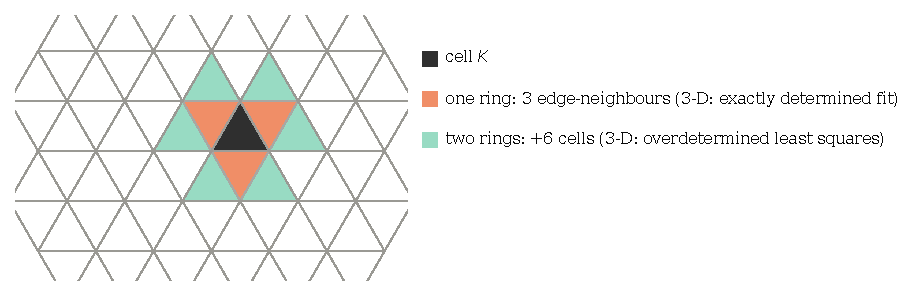
\includegraphics[width=\textwidth]{figures/fig_schematic.pdf}
  \caption{Schematic, two-dimensional analogue of the recovery neighbourhoods. In three
  dimensions the one-ring star has $16$ faces and $5$ closure relations, so the closed
  linear fit (eleven unknowns) is exactly determined. The two-ring neighbourhood
  oversamples it.}
  \label{fig:schematic}
\end{figure}

\begin{figure}[t]
  \centering
  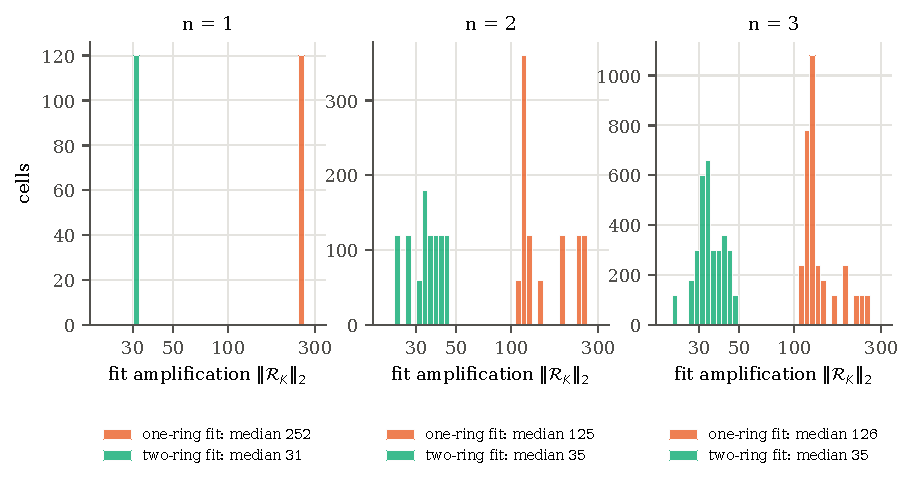
\includegraphics[width=\textwidth]{figures/fig_conditioning.pdf}
  \caption{Per-cell amplification $\norm{\cR_K}_2$ of the curvature recovery, from
  neighbourhood fluxes to the eleven coefficients. The one-ring recovery is exactly
  determined; the two-ring recovery is overdetermined and its amplification is lower and
  mesh-uniform.}
  \label{fig:conditioning}
\end{figure}

\section{Results}\label{sec:results}

All numbers below were recomputed from the frozen inputs by the scripts accompanying this
paper. The original Whitney and one-ring numbers reproduce the earlier reports to every
printed digit; for example $29.8111\%$ and $4.8414\%$ at $n=1$.

\paragraph{Convergence.}
Table~\ref{tab:force} and Figure~\ref{fig:force} give the relative force error.
\begin{itemize}
  \item The two-ring Petrov--Galerkin force falls from $6.22\%$ to $1.45\%$, with observed
    orders $0.73$, $0.80$ and $1.29$, and passes the unchanged \BW{} gate.
  \item The $q4$/$q6$ velocity differences are $2.3\times10^{-7}$, $8.2\times10^{-9}$,
    $1.4\times10^{-9}$ and $1.0\times10^{-10}$, at least five orders below the error.
  \item The solver corrections are of order $10^{-12}$.
\end{itemize}
The two-ring error is slightly above the one-ring error at every level ($1.45\%$ vs.\
$1.17\%$ at $n=5$), a modest price for stability. The recovered curvature itself
converges at second order (Figure~\ref{fig:curvature}), reaching $0.155\%$ at $n=5$,
against Whitney's first-order $1.53\%$.

\begin{table}[t]\centering\small
\caption{Relative instantaneous force error $\varepsilon_n$ (\%, $q6$). Orders are observed orders between consecutive levels, computed as in \BW{} from the absolute mass-norm error. The two-ring Petrov--Galerkin column passes \BW{} as evaluated by the unchanged gate function.}
\label{tab:force}
\begin{tabular}{rrrrrrrrr}\toprule
$n$ & $h_{\max}$ & Whitney & PG 1-ring & order & \textbf{PG 2-ring} & \textbf{order} & Var.\ 1-ring & Var.\ 2-ring \\ \midrule
1 & 0.3881 & 29.81 & 4.84 &  & \textbf{6.22} &  & 58.2 & 45.4 \\
2 & 0.2017 & 25.98 & 3.55 & 0.46 & \textbf{3.83} & \textbf{0.73} & 663.4 & 276.3 \\
3 & 0.1355 & 25.86 & 2.30 & 1.09 & \textbf{2.79} & \textbf{0.80} & 778.3 & 330.2 \\
5 & 0.0816 & 26.13 & 1.17 & 1.33 & \textbf{1.45} & \textbf{1.29} & --- & --- \\
\midrule
\multicolumn{9}{l}{Two-ring gate: \texttt{pass}=true; $q4/q6$ differences 2.3e-07--1.0e-10; solver corrections $\le$ 4.1e-12.}\\
\bottomrule\end{tabular}\end{table}


\begin{figure}[t]
  \centering
  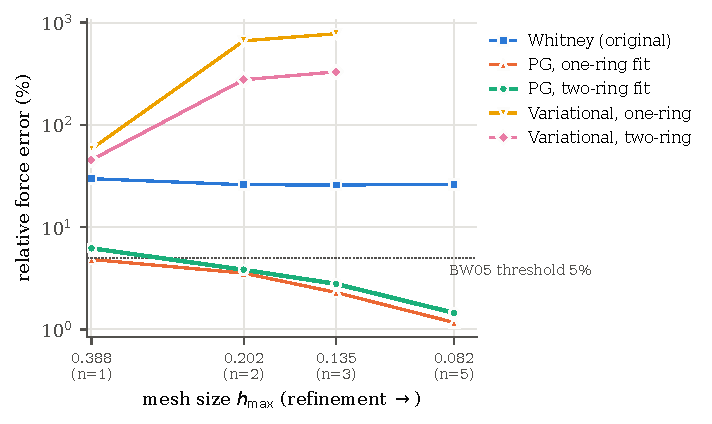
\includegraphics[width=0.98\textwidth]{figures/fig_force_error.pdf}
  \caption{Relative instantaneous force error under refinement. Whitney floors near
  $26\%$. Both Petrov--Galerkin forces converge, and the variational force of the same
  recovery diverges.}
  \label{fig:force}
\end{figure}

\begin{figure}[t]
  \centering
  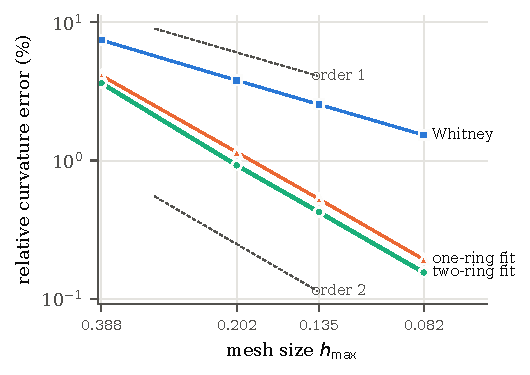
\includegraphics[width=0.6\textwidth]{figures/fig_curvature_error.pdf}
  \caption{Relative curvature error of the trial field. Whitney converges at first order;
  both recoveries at second order, as Lemma~\ref{lem:acc} predicts.}
  \label{fig:curvature}
\end{figure}

\paragraph{Stability.}
Table~\ref{tab:stability} and Figure~\ref{fig:spectra} give the two stability measures.
\begin{itemize}
  \item \emph{S3.} With two rings, the number of small eigenvalues equals the Whitney
    gauge dimension ($21$, $163$, $545$), and every physical eigenvalue has positive real
    part. The smallest real parts are $4.001$, $3.994$ and $3.997$, the control's
    eigenvalue $\delta dA=4A$; Whitney's are $4.017$, $4.005$ and $4.002$.
  \item \emph{Numerical range.} We also report the stronger certificate: the smallest
    eigenvalue of the symmetric part $\tfrac12(K_{\mathrm{PG}}+K_{\mathrm{PG}}^\top)$
    against $B_h$, restricted to the physical (non-gauge) space.
\end{itemize}

\begin{proposition}[Dissipativity]\label{prop:diss}
If $\tfrac12(K+K^\top)\succeq\mu B_h$ on the physical space with $\mu>0$, then every
solution of $B_h\dot a=-Ka$ satisfies $\norm{a(t)}_{B_h}\le e^{-\mu t}\norm{a(0)}_{B_h}$
there. In particular there is no transient non-normal growth.
\end{proposition}
\begin{proof}
$\tfrac{d}{dt}\tfrac12\norm{a}_{B_h}^2=-a^\top Ka=-a^\top\tfrac12(K+K^\top)a\le-\mu\norm{a}_{B_h}^2$.
\end{proof}

With two rings, $\mu=3.998$ at $n=1$ and $\mu=3.969$ at $n=2$. With one ring, the
symmetric part is indefinite, with $70$ and $472$ negative directions and minima of
$-1.35\times10^{4}$ and $-2.42\times10^{4}$.

\begin{table}[t]\centering\small
\caption{Stability. S3: generalized spectrum of $(K_{\mathrm{PG}},B_h)$; ``gauge'' counts eigenvalues of modulus below one (Whitney / PG). $\mu$: smallest eigenvalue of the symmetric part against $B_h$ on the physical space (Proposition~\ref{prop:diss}). Dashes: not decomposed.}
\label{tab:stability}
\begin{tabular}{rr rr rr rr}\toprule
 & & \multicolumn{2}{c}{min Re $\lambda$} & \multicolumn{2}{c}{\# Re $\lambda<0$} & \multicolumn{2}{c}{$\mu$} \\
\cmidrule(lr){3-4}\cmidrule(lr){5-6}\cmidrule(lr){7-8}
$n$ & gauge & 1-ring & \textbf{2-ring} & 1-ring & \textbf{2-ring} & 1-ring & \textbf{2-ring} \\ \midrule
1 & 21/21 & -13479 & \textbf{4.001} & 70 & \textbf{0} & -13512 & \textbf{3.998} \\
2 & 163/163 & -23940 & \textbf{3.994} & 489 & \textbf{0} & -24227 & \textbf{3.969} \\
3 & 545/545 & --- & \textbf{3.997} & --- & \textbf{0} & --- & --- \\
\bottomrule\end{tabular}\end{table}


\begin{figure}[t]
  \centering
  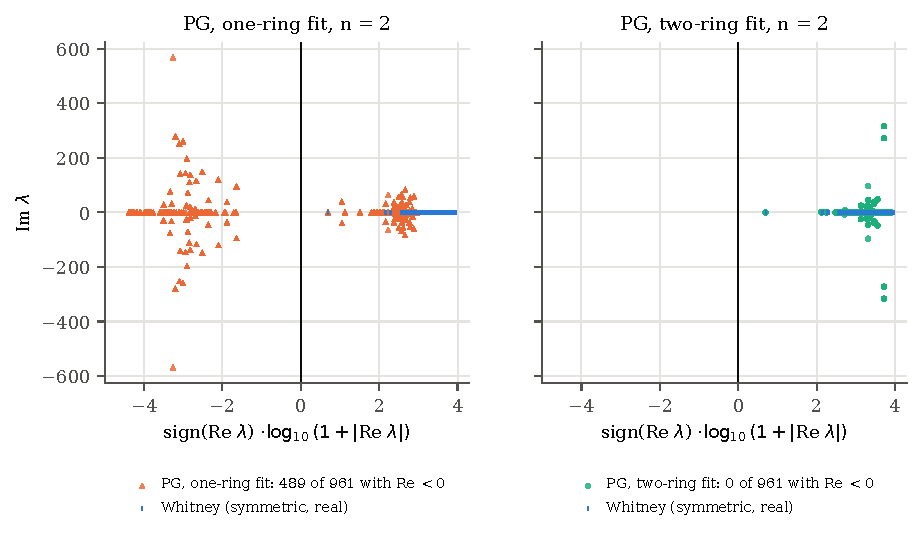
\includegraphics[width=\textwidth]{figures/fig_spectra.pdf}
  \caption{Generalized spectra of $(K_{\mathrm{PG}},B_h)$ at $n=2$; the real axis is
  signed-logarithmic. One ring: many rough modes with large negative real part. Two
  rings: every physical eigenvalue in the right half-plane, and the real extent matches
  the Whitney spectrum (ticks).}
  \label{fig:spectra}
\end{figure}

\section{Mechanism removals, and the variational question}\label{sec:removals}

Each ingredient was removed in turn, on the same data and with the same measurement
(Table~\ref{tab:removals}):
\begin{itemize}
  \item Removing the second ring restores the exactly determined fit, and S3 fails.
  \item Replacing the recovered trial by the Whitney trial restores the $26\%$ floor.
  \item Replacing the Whitney test by the recovered test gives the variational force,
    which diverges ($45\%$ and $276\%$ at $n=1,2$ with two rings; $58\%$, $663\%$ and
    $778\%$ with one).
\end{itemize}

The natural symmetric repair is the operator $K_{\mathrm{PG}}+K_{\mathrm{PG}}^\top-K_W$,
the Hessian of the energy linearized in the recovery. It equals $K_{\mathrm{PG}}$ plus
the transpose term $D^\top(\cR-j)^\top Hj\,D$. By~\eqref{eq:decomp}, that term is
precisely a test-variation defect, and Table~\ref{tab:removals} shows it growing under
refinement for both ring counts. A force derived from an energy therefore needs a
recovery whose \emph{transpose} preserves the Whitney moments of smooth fields:
\[
  \cR^\top Hc_F \approx j^\top Hc_F.
\]
That is a column-wise condition. Imposing it exactly, together with row-wise
exactness~\eqref{eq:fit}, couples every face to every cell whose neighbourhood contains
it. In an exploratory construction we found this coupling solvable but dense, and we
leave a scalable formulation open.

\begin{table}[t]\centering\small
\caption{Mechanism removals: relative force error (\%) at $n=1,2$ (and $n=5$ where measured). ``Transpose term'' is $D^\top(\cR-j)^\top Hj\,Da$, measured in the same norm.}
\label{tab:removals}
\begin{tabular}{l rrr l}\toprule
Variant & $n=1$ & $n=2$ & $n=5$ & Fails \\ \midrule
Two-ring Petrov--Galerkin (this work) & 6.22 & 3.83 & 1.45 & --- \\
$-$ second ring (one-ring PG) & 4.84 & 3.55 & 1.17 & S3 \\
$-$ recovered trial (Whitney) & 29.81 & 25.98 & 26.13 & \BW{} floor \\
$-$ Whitney test (variational, 2-ring) & 45.4 & 276.3 & --- & \BW{}, diverges \\
$-$ Whitney test (variational, 1-ring) & 58.2 & 663.4 & --- & \BW{}, diverges \\
Symmetrized $K_{\mathrm{PG}}+K_{\mathrm{PG}}^\top-K_W$, 2-ring & 23.0 & 276.5 & --- & \BW{} \\
\quad transpose term alone, 2-ring & 19.7 & 275.6 & --- & \\
Symmetrized, 1-ring & 64.8 & 671.3 & --- & \BW{} \\
\quad transpose term alone, 1-ring & 61.2 & 669.8 & --- & \\
\bottomrule\end{tabular}\end{table}


\section{Discussion}

The central observation is simple to state. \emph{The Petrov--Galerkin force was never
inconsistent; it was ill-conditioned.} The one-ring recovery is the minimal-information
choice, and it has no choice but to read every rough flux pattern as a linear field. Once
the recovery is given more information than it strictly needs, rough patterns are
averaged rather than interpolated. Exactness on the model space is untouched, so
consistency survives. Stability follows without any damping parameter, filter or
regularization: the only change is a neighbourhood radius, and only radii one and two
were ever run.

In \DAVIS{} terms, this is the geometry-first principle applied to the discretization
itself. A well-posed geometric statistic needs a representation whose distortion is
controlled on the relevant path family. Here the relevant family is the space of all
discrete variations, rough ones included, and the controlled quantity is the
amplification $\Lambda$.

\paragraph{Limitations.}
\begin{itemize}
  \item The results concern a single Abelian control on a single round quotient; the
    Berger metrics, the full $SU(2)$ nonlinearity and time integration are untested.
  \item The S3 spectrum is decomposed at $n\le 3$ and the numerical range at $n\le 2$;
    the finest level is not decomposed.
  \item The observed orders $0.73$ and $0.80$ before the last refinement are only
    moderately above the threshold, and a further level would strengthen the rate claim.
  \item The force is not the gradient of an energy. Whether a dissipative, consistent,
    non-variational force suffices for the programme's purposes is a modelling decision,
    not a numerical one.
  \item No Ricci-flow claim is made. The target here is the Abelian Yang--Mills force
    $-\delta dA$; the result is a prerequisite for a lattice \DAVIS{}--Wilson
    correspondence, not an instance of one.
\end{itemize}

\paragraph{Reproducibility.}
The recovery is \texttt{scripts/ricci\_pg\_tworing.py}; the gate and stability harness
is \texttt{scripts/ricci\_pg\_tworing\_gate.py}; focused tests are in
\texttt{scripts/test\_ricci\_pg\_tworing.py}. Every number and figure in this paper is
regenerated by \texttt{make\_data.py}, \texttt{numerical\_range.py} and
\texttt{make\_figures.py} in the paper's directory, and every table by
\texttt{make\_tables.py}, all from the frozen, hash-checked inputs of the
\GIGI{} Ricci checkpoint.

\paragraph{Acknowledgements.}
The computations, code and a first draft of this manuscript were produced with
substantial assistance from AI research agents (Anthropic's Claude), working under the
author's direction across several sessions. The one-ring Petrov--Galerkin recovery and
its mechanism-removal programme came from one such session; the conditioning diagnosis
and the two-ring recovery from another.

\begin{thebibliography}{99}\small
\bibitem{afgt2014} D.~N.~Arnold, R.~S.~Falk, J.~Guzm\'an, G.~Tsogtgerel, On the consistency of the combinatorial codifferential, \emph{Trans.\ Amer.\ Math.\ Soc.} 366 (2014) 5487--5502.
\bibitem{afw2006} D.~N.~Arnold, R.~S.~Falk, R.~Winther, Finite element exterior calculus, homological techniques, and applications, \emph{Acta Numerica} 15 (2006) 1--155.
\bibitem{afw2010} D.~N.~Arnold, R.~S.~Falk, R.~Winther, Finite element exterior calculus: from Hodge theory to numerical stability, \emph{Bull.\ Amer.\ Math.\ Soc.} 47 (2010) 281--354.
\bibitem{bossavit1988} A.~Bossavit, Whitney forms: a class of finite elements for three-dimensional computations in electromagnetism, \emph{IEE Proc.\ A} 135 (1988) 493--500.
\bibitem{cdl2013} A.~Cohen, M.~A.~Davenport, D.~Leviatan, On the stability and accuracy of least squares approximations, \emph{Found.\ Comput.\ Math.} 13 (2013) 819--834.
\bibitem{hiptmair2002} R.~Hiptmair, Finite elements in computational electromagnetism, \emph{Acta Numerica} 11 (2002) 237--339.
\bibitem{whitney1957} H.~Whitney, \emph{Geometric Integration Theory}, Princeton University Press, 1957.
\bibitem{zz1992} O.~C.~Zienkiewicz, J.~Z.~Zhu, The superconvergent patch recovery and a posteriori error estimates, \emph{Int.\ J.\ Numer.\ Methods Eng.} 33 (1992) 1331--1364.
\end{thebibliography}

\end{document}
